\newpage
\section{Components Used}

\subsection{Accelerometer}
The MPU-6050 is a popular integrated circuit that combines a 3-axis gyroscope and a 3-axis accelerometer into a single chip. It's commonly used in various applications, particularly in motion sensing, orientation tracking, and gesture recognition systems.
For precision tracking of both fast and slow motions, the MPU-60X0 features a user-programmable gyroscope full-scale range of ±250, ±500, ±1000, and ±2000°/sec (dps). The parts also have a user-programmable accelerometer full-scale range of ±2g, ±4g, ±8g, and ±16g. The typical operating voltage range is 2.375V to 3.46V with operating current 100µA.
\begin{figure}[H]
    \centering
    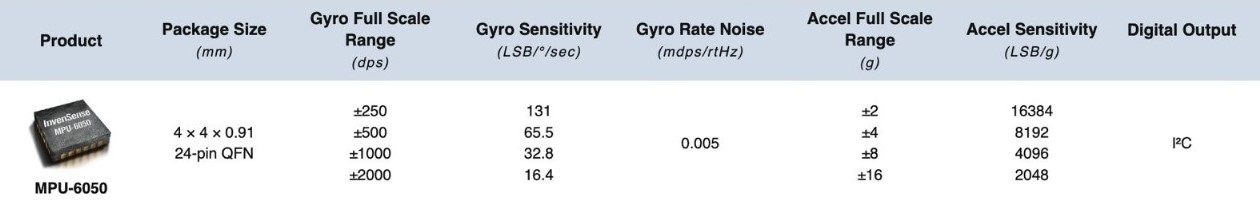
\includegraphics[width=1\linewidth]{Files/Images/Accelerometer.jpg}
    \caption{MPU 6050 Details}
    \label{fig:enter-label}
\end{figure}

\subsection{MAX7219/MAX7221}
\subsubsection*{Description}
The MAX7219/MAX7221 are small display drivers with serial input/output capability. They connect microprocessors ($\mu$Ps) to 7-segment numeric LED displays with a maximum of 8 digits, bar-graph displays, or 64 separate displays.

Light-emitting diodes. The integrated circuit contains a BCD code-B decoder, multiplex scan circuitry, segment and digit drivers, and an 8x8 static RAM that saves each digit. A single external resistor is sufficient to establish the segment current for all LEDs. The MAX7221 is compatible with \gls{SPI}™, \gls{QSPI}™, and \gls{MICROWIRE}™ communication protocols. It is equipped with segment drivers that have low slew rates to minimize electromagnetic interference (EMI).
The device features a practical 4-wire serial interface that can be easily connected to any standard microprocessors. Each individual digit can be targeted and modified without having to rewrite the entire display. The MAX7219/MAX7221 additionally provide the user with the option to choose between code-B decoding or no-decode for each digit.
The devices are equipped with a low-power shutdown mode that consumes only $\SI{150}{\mu A}$, as well as analog and digital brightness control. They also have a scan-limit register, which enables the user to display anywhere from 1 to 8 digits. Additionally, there is a test mode available that activates all LEDs simultaneously.{\tiny \textcolor{white}{\ac{SPI}}}{\tiny \textcolor{white}{\ac{QSPI}}}
\subsubsection*{Features}
\begin{itemize}
    \item $\SI{10}{MHz}$ Serial Interface
    \item Individual LED Segment Control
    \item Decode/No-Decode Digit Selection
    \item $\SI{150}{\mu A}$ Low-Power Shutdown (Data Retained)
    \item Digital and Analog Brightness Control
    \item Display Blanked on Power-Up
    \item Drive Common-Cathode LED Display
    \item Slew-Rate Limited Segment Drivers
for Lower EMI (MAX7221)
    \item SPI, QSPI, MICROWIRE Serial Interface (MAX7221)
    \item 24-Pin DIP and SO Packages
\end{itemize}

\begin{figure}[H]
    \centering
    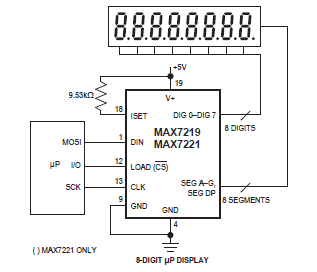
\includegraphics[width=0.7\textwidth]{Files/Images/Max7219.png}
    \caption{Typical Application of \textbf{MAX7219/MAX7221}}
    \label{Max7219}
\end{figure}


\begin{figure}[H]
\centering

\begin{tikzpicture}[node distance=3cm, on grid, auto, thick, initial text=]

    % Define the states
    \node[state, initial] (A) {Counter};
    \node[state, right=of A] (B) {OOS};

    % Draw the transitions
    \path[->]
        (A) edge[loop above] node {X} (A)
        (A) edge[bend left] node {B} (B)
        (B) edge[loop above] node {X} (B)
        (B) edge[bend left] node {A} (A);

\end{tikzpicture}
\caption{FSM diagram for the display}
\end{figure}